% 角平分线逆定理：PM⊥OA, PN⊥OB, PM=PN → OP 平分 ∠AOB
\documentclass[tikz,border=4pt]{standalone}
\usepackage{ctex}
\usepackage{amsmath}
\usetikzlibrary{calc, decorations.markings}
\begin{document}
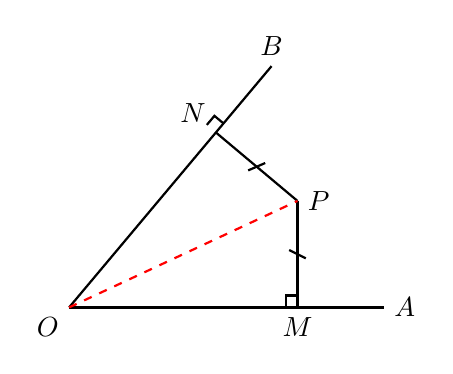
\begin{tikzpicture}[scale=1.0, thick,
  tick/.style={postaction={decorate, decoration={markings,
    mark=at position 0.5 with {\draw (-1.5pt,-3pt) -- (1.5pt,3pt);}}}}]
  \coordinate (O) at (0,0);
  \coordinate (A) at (4, 0);                % OA 沿 x 轴
  \coordinate (B) at ({4*cos(50)}, {4*sin(50)}); % OB 在上方 50°

  \draw (O) -- (A);
  \draw (O) -- (B);

  % P 在角平分线上 (角 25°), 距 O = 3.2
  \coordinate (P) at ({3.2*cos(25)}, {3.2*sin(25)});
  % PM ⊥ OA: M 是 P 在 x 轴上投影
  \coordinate (M) at ({3.2*cos(25)}, 0);
  % PN ⊥ OB: N 是 P 在 OB 上垂足
  % OB 方向 (cos50, sin50), 投影长度 = P·OB方向
  \pgfmathsetmacro{\proj}{3.2*cos(25)*cos(50)+3.2*sin(25)*sin(50)}
  \coordinate (N) at ({\proj*cos(50)}, {\proj*sin(50)});

  \draw[tick] (P) -- (M);
  \draw[tick] (P) -- (N);
  \draw[red, dashed] (O) -- (P);

  % 直角符号
  \draw ($(M)+(-0.15,0)$) -- ($(M)+(-0.15,0.15)$) -- ($(M)+(0,0.15)$);
  % 在 N 处直角符号
  \pgfmathsetmacro{\nx}{\proj*cos(50)}
  \pgfmathsetmacro{\ny}{\proj*sin(50)}
  \draw ($(N)+({0.15*cos(140)}, {0.15*sin(140)})$)
     -- ($(N)+({0.15*cos(140)+0.15*cos(50)}, {0.15*sin(140)+0.15*sin(50)})$)
     -- ($(N)+({0.15*cos(50)}, {0.15*sin(50)})$);

  \node[below left] at (O) {$O$};
  \node[right]      at (A) {$A$};
  \node[above]      at (B) {$B$};
  \node[right]      at (P) {$P$};
  \node[below]      at (M) {$M$};
  \node[above left] at (N) {$N$};
\end{tikzpicture}
\end{document}
